\documentclass[twoside]{book}

% Packages required by doxygen
\usepackage{fixltx2e}
\usepackage{calc}
\usepackage{doxygen}
\usepackage[export]{adjustbox} % also loads graphicx
\usepackage{graphicx}
\usepackage[utf8]{inputenc}
\usepackage{makeidx}
\usepackage{multicol}
\usepackage{multirow}
\PassOptionsToPackage{warn}{textcomp}
\usepackage{textcomp}
\usepackage[nointegrals]{wasysym}
\usepackage[table]{xcolor}

% Font selection
\usepackage[T1]{fontenc}
\usepackage[scaled=.90]{helvet}
\usepackage{courier}
\usepackage{amssymb}
\usepackage{sectsty}
\renewcommand{\familydefault}{\sfdefault}
\allsectionsfont{%
  \fontseries{bc}\selectfont%
  \color{darkgray}%
}
\renewcommand{\DoxyLabelFont}{%
  \fontseries{bc}\selectfont%
  \color{darkgray}%
}
\newcommand{\+}{\discretionary{\mbox{\scriptsize$\hookleftarrow$}}{}{}}

% Page & text layout
\usepackage{geometry}
\geometry{%
  a4paper,%
  top=2.5cm,%
  bottom=2.5cm,%
  left=2.5cm,%
  right=2.5cm%
}
\tolerance=750
\hfuzz=15pt
\hbadness=750
\setlength{\emergencystretch}{15pt}
\setlength{\parindent}{0cm}
\setlength{\parskip}{3ex plus 2ex minus 2ex}
\makeatletter
\renewcommand{\paragraph}{%
  \@startsection{paragraph}{4}{0ex}{-1.0ex}{1.0ex}{%
    \normalfont\normalsize\bfseries\SS@parafont%
  }%
}
\renewcommand{\subparagraph}{%
  \@startsection{subparagraph}{5}{0ex}{-1.0ex}{1.0ex}{%
    \normalfont\normalsize\bfseries\SS@subparafont%
  }%
}
\makeatother

% Headers & footers
\usepackage{fancyhdr}
\pagestyle{fancyplain}
\fancyhead[LE]{\fancyplain{}{\bfseries\thepage}}
\fancyhead[CE]{\fancyplain{}{}}
\fancyhead[RE]{\fancyplain{}{\bfseries\leftmark}}
\fancyhead[LO]{\fancyplain{}{\bfseries\rightmark}}
\fancyhead[CO]{\fancyplain{}{}}
\fancyhead[RO]{\fancyplain{}{\bfseries\thepage}}
\fancyfoot[LE]{\fancyplain{}{}}
\fancyfoot[CE]{\fancyplain{}{}}
\fancyfoot[RE]{\fancyplain{}{\bfseries\scriptsize Generated by Doxygen }}
\fancyfoot[LO]{\fancyplain{}{\bfseries\scriptsize Generated by Doxygen }}
\fancyfoot[CO]{\fancyplain{}{}}
\fancyfoot[RO]{\fancyplain{}{}}
\renewcommand{\footrulewidth}{0.4pt}
\renewcommand{\chaptermark}[1]{%
  \markboth{#1}{}%
}
\renewcommand{\sectionmark}[1]{%
  \markright{\thesection\ #1}%
}

% Indices & bibliography
\usepackage{natbib}
\usepackage[titles]{tocloft}
\setcounter{tocdepth}{3}
\setcounter{secnumdepth}{5}
\makeindex

% Hyperlinks (required, but should be loaded last)
\usepackage{ifpdf}
\ifpdf
  \usepackage[pdftex,pagebackref=true]{hyperref}
\else
  \usepackage[ps2pdf,pagebackref=true]{hyperref}
\fi
\hypersetup{%
  colorlinks=true,%
  linkcolor=blue,%
  citecolor=blue,%
  unicode%
}

% Custom commands
\newcommand{\clearemptydoublepage}{%
  \newpage{\pagestyle{empty}\cleardoublepage}%
}

\usepackage{caption}
\captionsetup{labelsep=space,justification=centering,font={bf},singlelinecheck=off,skip=4pt,position=top}

%===== C O N T E N T S =====

\begin{document}

% Titlepage & ToC
\hypersetup{pageanchor=false,
             bookmarksnumbered=true,
             pdfencoding=unicode
            }
\pagenumbering{roman}
\begin{titlepage}
\vspace*{7cm}
\begin{center}%
{\Large Simple J\+S\+ON \\[1ex]\large 0.\+1 }\\
\vspace*{1cm}
{\large Generated by Doxygen 1.8.11}\\
\end{center}
\end{titlepage}
\clearemptydoublepage
\tableofcontents
\clearemptydoublepage
\pagenumbering{arabic}
\hypersetup{pageanchor=true}

%--- Begin generated contents ---
\chapter{Data Structure Index}
\section{Data Structures}
Here are the data structures with brief descriptions\+:\begin{DoxyCompactList}
\item\contentsline{section}{\hyperlink{structjsParse}{js\+Parse} \\*Structure keeps track of the buffer being parsed and the position last used }{\pageref{d9/dd9/structjsParse}}{}
\item\contentsline{section}{\hyperlink{structSJList}{S\+J\+List} \\*This is a simple list structure intended to hold an arbitrary number of elements list will automatically grow as space is needed to accomodate more elements }{\pageref{d9/d7e/structSJList}}{}
\item\contentsline{section}{\hyperlink{structSJListElementData}{S\+J\+List\+Element\+Data} \\*Simple datatype abstracting the data held }{\pageref{d0/d8b/structSJListElementData}}{}
\item\contentsline{section}{\hyperlink{structSJPair}{S\+J\+Pair} \\*Object is a list of key/value pairs }{\pageref{dd/d6d/structSJPair}}{}
\item\contentsline{section}{\hyperlink{structSJson__S}{S\+Json\+\_\+S} \\*This is the abstract container structure for all json data This structure may be an object, array, string, null, boolean value, integer or float }{\pageref{d9/dca/structSJson__S}}{}
\item\contentsline{section}{\hyperlink{structSJString}{S\+J\+String} \\*Basic structure that keeps track of a string and its length Automatically grows to accomodate longer strings }{\pageref{d4/d1f/structSJString}}{}
\end{DoxyCompactList}

\chapter{Data Structure Documentation}
\hypertarget{structjsParse}{}\section{js\+Parse Struct Reference}
\label{structjsParse}\index{js\+Parse@{js\+Parse}}


structure keeps track of the buffer being parsed and the position last used  


\subsection*{Data Fields}
\begin{DoxyCompactItemize}
\item 
char $\ast$ \hyperlink{structjsParse_a9c0b007595634aae8cdb98a7a85b846a}{buffer}
\item 
char $\ast$ \hyperlink{structjsParse_ace05b203435af05113a9a4b7c40f0324}{position}
\item 
char $\ast$ \hyperlink{structjsParse_aa9b5c5a2d56b1753ccadf84c00385fba}{end}
\end{DoxyCompactItemize}


\subsection{Detailed Description}
structure keeps track of the buffer being parsed and the position last used 

Definition at line 13 of file simple\+\_\+json\+\_\+parse.\+c.



\subsection{Field Documentation}
\index{js\+Parse@{js\+Parse}!buffer@{buffer}}
\index{buffer@{buffer}!js\+Parse@{js\+Parse}}
\subsubsection[{\texorpdfstring{buffer}{buffer}}]{\setlength{\rightskip}{0pt plus 5cm}char$\ast$ js\+Parse\+::buffer}\hypertarget{structjsParse_a9c0b007595634aae8cdb98a7a85b846a}{}\label{structjsParse_a9c0b007595634aae8cdb98a7a85b846a}
the buffer being parsed 

Definition at line 15 of file simple\+\_\+json\+\_\+parse.\+c.

\index{js\+Parse@{js\+Parse}!end@{end}}
\index{end@{end}!js\+Parse@{js\+Parse}}
\subsubsection[{\texorpdfstring{end}{end}}]{\setlength{\rightskip}{0pt plus 5cm}char$\ast$ js\+Parse\+::end}\hypertarget{structjsParse_aa9b5c5a2d56b1753ccadf84c00385fba}{}\label{structjsParse_aa9b5c5a2d56b1753ccadf84c00385fba}
the last position to prevent over seek 

Definition at line 17 of file simple\+\_\+json\+\_\+parse.\+c.

\index{js\+Parse@{js\+Parse}!position@{position}}
\index{position@{position}!js\+Parse@{js\+Parse}}
\subsubsection[{\texorpdfstring{position}{position}}]{\setlength{\rightskip}{0pt plus 5cm}char$\ast$ js\+Parse\+::position}\hypertarget{structjsParse_ace05b203435af05113a9a4b7c40f0324}{}\label{structjsParse_ace05b203435af05113a9a4b7c40f0324}
the current position being parsed 

Definition at line 16 of file simple\+\_\+json\+\_\+parse.\+c.



The documentation for this struct was generated from the following file\+:\begin{DoxyCompactItemize}
\item 
/home/djkehoe/git/simple\+\_\+json/src/simple\+\_\+json\+\_\+parse.\+c\end{DoxyCompactItemize}

\hypertarget{structSJList}{}\section{S\+J\+List Struct Reference}
\label{structSJList}\index{S\+J\+List@{S\+J\+List}}


this is a simple list structure intended to hold an arbitrary number of elements list will automatically grow as space is needed to accomodate more elements  




{\ttfamily \#include $<$simple\+\_\+json\+\_\+list.\+h$>$}



Collaboration diagram for S\+J\+List\+:
\nopagebreak
\begin{figure}[H]
\begin{center}
\leavevmode
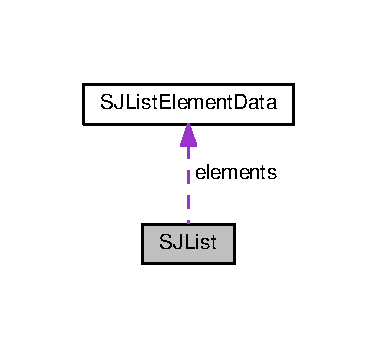
\includegraphics[width=181pt]{d5/d2e/structSJList__coll__graph}
\end{center}
\end{figure}
\subsection*{Data Fields}
\begin{DoxyCompactItemize}
\item 
\hyperlink{structSJListElementData}{S\+J\+List\+Element\+Data} $\ast$ \hyperlink{structSJList_a43fc72ebe9774607d3c503917b911c7c}{elements}
\item 
unsigned int \hyperlink{structSJList_a1e3944d88b5e2aac09698498f376559b}{size}
\item 
unsigned int \hyperlink{structSJList_a706017d74f3cde16157127d8e8025116}{count}
\end{DoxyCompactItemize}


\subsection{Detailed Description}
this is a simple list structure intended to hold an arbitrary number of elements list will automatically grow as space is needed to accomodate more elements 

Definition at line 16 of file simple\+\_\+json\+\_\+list.\+h.



\subsection{Field Documentation}
\index{S\+J\+List@{S\+J\+List}!count@{count}}
\index{count@{count}!S\+J\+List@{S\+J\+List}}
\subsubsection[{\texorpdfstring{count}{count}}]{\setlength{\rightskip}{0pt plus 5cm}unsigned int S\+J\+List\+::count}\hypertarget{structSJList_a706017d74f3cde16157127d8e8025116}{}\label{structSJList_a706017d74f3cde16157127d8e8025116}
how many elements are in use 

Definition at line 20 of file simple\+\_\+json\+\_\+list.\+h.

\index{S\+J\+List@{S\+J\+List}!elements@{elements}}
\index{elements@{elements}!S\+J\+List@{S\+J\+List}}
\subsubsection[{\texorpdfstring{elements}{elements}}]{\setlength{\rightskip}{0pt plus 5cm}{\bf S\+J\+List\+Element\+Data}$\ast$ S\+J\+List\+::elements}\hypertarget{structSJList_a43fc72ebe9774607d3c503917b911c7c}{}\label{structSJList_a43fc72ebe9774607d3c503917b911c7c}
a pointer to the array of the data 

Definition at line 18 of file simple\+\_\+json\+\_\+list.\+h.

\index{S\+J\+List@{S\+J\+List}!size@{size}}
\index{size@{size}!S\+J\+List@{S\+J\+List}}
\subsubsection[{\texorpdfstring{size}{size}}]{\setlength{\rightskip}{0pt plus 5cm}unsigned int S\+J\+List\+::size}\hypertarget{structSJList_a1e3944d88b5e2aac09698498f376559b}{}\label{structSJList_a1e3944d88b5e2aac09698498f376559b}
how much memory has been allocated 

Definition at line 19 of file simple\+\_\+json\+\_\+list.\+h.



The documentation for this struct was generated from the following file\+:\begin{DoxyCompactItemize}
\item 
/home/djkehoe/git/simple\+\_\+json/include/simple\+\_\+json\+\_\+list.\+h\end{DoxyCompactItemize}

\hypertarget{structSJListElementData}{}\section{S\+J\+List\+Element\+Data Struct Reference}
\label{structSJListElementData}\index{S\+J\+List\+Element\+Data@{S\+J\+List\+Element\+Data}}


simple datatype abstracting the data held.  




{\ttfamily \#include $<$simple\+\_\+json\+\_\+list.\+h$>$}

\subsection*{Data Fields}
\begin{DoxyCompactItemize}
\item 
void $\ast$ \hyperlink{structSJListElementData_ae48c7175a4477eb042b02b70c88485d1}{data}
\end{DoxyCompactItemize}


\subsection{Detailed Description}
simple datatype abstracting the data held. 

Definition at line 7 of file simple\+\_\+json\+\_\+list.\+h.



\subsection{Field Documentation}
\index{S\+J\+List\+Element\+Data@{S\+J\+List\+Element\+Data}!data@{data}}
\index{data@{data}!S\+J\+List\+Element\+Data@{S\+J\+List\+Element\+Data}}
\subsubsection[{\texorpdfstring{data}{data}}]{\setlength{\rightskip}{0pt plus 5cm}void$\ast$ S\+J\+List\+Element\+Data\+::data}\hypertarget{structSJListElementData_ae48c7175a4477eb042b02b70c88485d1}{}\label{structSJListElementData_ae48c7175a4477eb042b02b70c88485d1}
pointer to the data being accessed 

Definition at line 9 of file simple\+\_\+json\+\_\+list.\+h.



The documentation for this struct was generated from the following file\+:\begin{DoxyCompactItemize}
\item 
/home/djkehoe/git/simple\+\_\+json/include/simple\+\_\+json\+\_\+list.\+h\end{DoxyCompactItemize}

\hypertarget{structSJPair}{}\section{S\+J\+Pair Struct Reference}
\label{structSJPair}\index{S\+J\+Pair@{S\+J\+Pair}}


an object is a list of key/value pairs  




Collaboration diagram for S\+J\+Pair\+:
\nopagebreak
\begin{figure}[H]
\begin{center}
\leavevmode
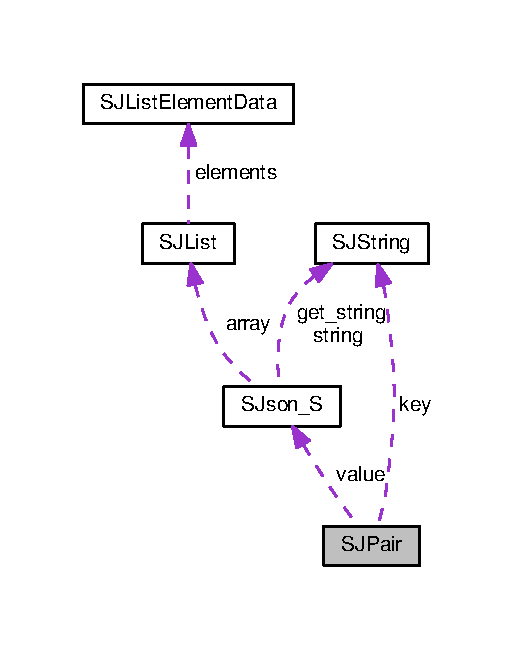
\includegraphics[width=248pt]{d7/d37/structSJPair__coll__graph}
\end{center}
\end{figure}
\subsection*{Data Fields}
\begin{DoxyCompactItemize}
\item 
\hyperlink{structSJString}{S\+J\+String} $\ast$ \hyperlink{structSJPair_a23681f167b9eac4d55be408c2007ae6c}{key}
\item 
\hyperlink{structSJson__S}{S\+Json} $\ast$ \hyperlink{structSJPair_aeee74c0e0e05940043b8aa96d1be43a4}{value}
\end{DoxyCompactItemize}


\subsection{Detailed Description}
an object is a list of key/value pairs 

Definition at line 24 of file simple\+\_\+json\+\_\+object.\+c.



\subsection{Field Documentation}
\index{S\+J\+Pair@{S\+J\+Pair}!key@{key}}
\index{key@{key}!S\+J\+Pair@{S\+J\+Pair}}
\subsubsection[{\texorpdfstring{key}{key}}]{\setlength{\rightskip}{0pt plus 5cm}{\bf S\+J\+String}$\ast$ S\+J\+Pair\+::key}\hypertarget{structSJPair_a23681f167b9eac4d55be408c2007ae6c}{}\label{structSJPair_a23681f167b9eac4d55be408c2007ae6c}
the identifying key 

Definition at line 26 of file simple\+\_\+json\+\_\+object.\+c.

\index{S\+J\+Pair@{S\+J\+Pair}!value@{value}}
\index{value@{value}!S\+J\+Pair@{S\+J\+Pair}}
\subsubsection[{\texorpdfstring{value}{value}}]{\setlength{\rightskip}{0pt plus 5cm}{\bf S\+Json}$\ast$ S\+J\+Pair\+::value}\hypertarget{structSJPair_aeee74c0e0e05940043b8aa96d1be43a4}{}\label{structSJPair_aeee74c0e0e05940043b8aa96d1be43a4}
the value the key references 

Definition at line 27 of file simple\+\_\+json\+\_\+object.\+c.



The documentation for this struct was generated from the following file\+:\begin{DoxyCompactItemize}
\item 
/home/djkehoe/git/simple\+\_\+json/src/simple\+\_\+json\+\_\+object.\+c\end{DoxyCompactItemize}

\hypertarget{structSJson__S}{}\section{S\+Json\+\_\+S Struct Reference}
\label{structSJson__S}\index{S\+Json\+\_\+S@{S\+Json\+\_\+S}}


this is the abstract container structure for all json data This structure may be an object, array, string, null, boolean value, integer or float  




{\ttfamily \#include $<$simple\+\_\+json\+\_\+value.\+h$>$}



Collaboration diagram for S\+Json\+\_\+S\+:
\nopagebreak
\begin{figure}[H]
\begin{center}
\leavevmode
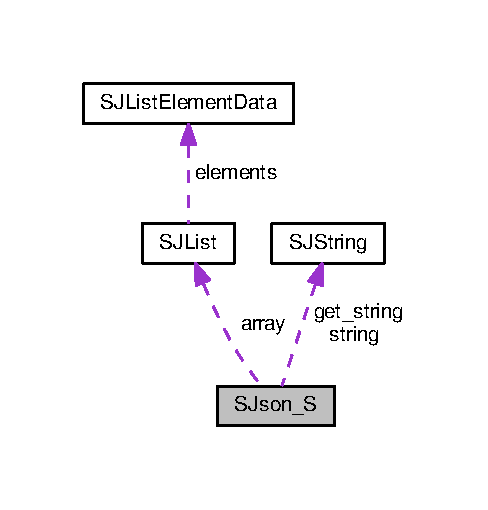
\includegraphics[width=234pt]{d2/d22/structSJson__S__coll__graph}
\end{center}
\end{figure}
\subsection*{Data Fields}
\begin{DoxyCompactItemize}
\item 
S\+J\+Value\+Types \hyperlink{structSJson__S_ad68edc13b2a814f9b920498ba439b8ba}{sjtype}
\item 
\begin{tabbing}
xx\=xx\=xx\=xx\=xx\=xx\=xx\=xx\=xx\=\kill
union \{\\
\>\hyperlink{structSJList}{SJList} $\ast$ \hyperlink{structSJson__S_aa8c595b7789550a64b08950b0ad88e1e}{array}\\
\>\hyperlink{structSJString}{SJString} $\ast$ \hyperlink{structSJson__S_ab50f7c395b214eb050ff59e3a9bbeb4a}{string}\\
\} \hyperlink{structSJson__S_a34c41be372d7bbe614b312cef2051b99}{v}\\

\end{tabbing}\item 
\hyperlink{structSJString}{S\+J\+String} $\ast$($\ast$ \hyperlink{structSJson__S_afd320740fab795e7063e89157a23c511}{get\+\_\+string} )(struct \hyperlink{structSJson__S}{S\+Json\+\_\+S} $\ast$json)
\item 
void($\ast$ \hyperlink{structSJson__S_a8bd24b6b85325a01b8bae6c5899583f2}{json\+\_\+free} )(struct \hyperlink{structSJson__S}{S\+Json\+\_\+S} $\ast$json)
\end{DoxyCompactItemize}


\subsection{Detailed Description}
this is the abstract container structure for all json data This structure may be an object, array, string, null, boolean value, integer or float 

Definition at line 19 of file simple\+\_\+json\+\_\+value.\+h.



\subsection{Field Documentation}
\index{S\+Json\+\_\+S@{S\+Json\+\_\+S}!array@{array}}
\index{array@{array}!S\+Json\+\_\+S@{S\+Json\+\_\+S}}
\subsubsection[{\texorpdfstring{array}{array}}]{\setlength{\rightskip}{0pt plus 5cm}{\bf S\+J\+List}$\ast$ S\+Json\+\_\+\+S\+::array}\hypertarget{structSJson__S_aa8c595b7789550a64b08950b0ad88e1e}{}\label{structSJson__S_aa8c595b7789550a64b08950b0ad88e1e}
an array or values or an array of pairs 

Definition at line 24 of file simple\+\_\+json\+\_\+value.\+h.

\index{S\+Json\+\_\+S@{S\+Json\+\_\+S}!get\+\_\+string@{get\+\_\+string}}
\index{get\+\_\+string@{get\+\_\+string}!S\+Json\+\_\+S@{S\+Json\+\_\+S}}
\subsubsection[{\texorpdfstring{get\+\_\+string}{get_string}}]{\setlength{\rightskip}{0pt plus 5cm}{\bf S\+J\+String}$\ast$($\ast$ S\+Json\+\_\+\+S\+::get\+\_\+string) (struct {\bf S\+Json\+\_\+S} $\ast$json)}\hypertarget{structSJson__S_afd320740fab795e7063e89157a23c511}{}\label{structSJson__S_afd320740fab795e7063e89157a23c511}
pointer to the function to convert this into json string 

Definition at line 27 of file simple\+\_\+json\+\_\+value.\+h.

\index{S\+Json\+\_\+S@{S\+Json\+\_\+S}!json\+\_\+free@{json\+\_\+free}}
\index{json\+\_\+free@{json\+\_\+free}!S\+Json\+\_\+S@{S\+Json\+\_\+S}}
\subsubsection[{\texorpdfstring{json\+\_\+free}{json_free}}]{\setlength{\rightskip}{0pt plus 5cm}void($\ast$ S\+Json\+\_\+\+S\+::json\+\_\+free) (struct {\bf S\+Json\+\_\+S} $\ast$json)}\hypertarget{structSJson__S_a8bd24b6b85325a01b8bae6c5899583f2}{}\label{structSJson__S_a8bd24b6b85325a01b8bae6c5899583f2}
pointer to the function to free this json 

Definition at line 28 of file simple\+\_\+json\+\_\+value.\+h.

\index{S\+Json\+\_\+S@{S\+Json\+\_\+S}!sjtype@{sjtype}}
\index{sjtype@{sjtype}!S\+Json\+\_\+S@{S\+Json\+\_\+S}}
\subsubsection[{\texorpdfstring{sjtype}{sjtype}}]{\setlength{\rightskip}{0pt plus 5cm}S\+J\+Value\+Types S\+Json\+\_\+\+S\+::sjtype}\hypertarget{structSJson__S_ad68edc13b2a814f9b920498ba439b8ba}{}\label{structSJson__S_ad68edc13b2a814f9b920498ba439b8ba}
internal tracking of the type. DO N\+OT T\+O\+U\+CH 

Definition at line 21 of file simple\+\_\+json\+\_\+value.\+h.

\index{S\+Json\+\_\+S@{S\+Json\+\_\+S}!string@{string}}
\index{string@{string}!S\+Json\+\_\+S@{S\+Json\+\_\+S}}
\subsubsection[{\texorpdfstring{string}{string}}]{\setlength{\rightskip}{0pt plus 5cm}{\bf S\+J\+String}$\ast$ S\+Json\+\_\+\+S\+::string}\hypertarget{structSJson__S_ab50f7c395b214eb050ff59e3a9bbeb4a}{}\label{structSJson__S_ab50f7c395b214eb050ff59e3a9bbeb4a}
the string if this is a string type 

Definition at line 25 of file simple\+\_\+json\+\_\+value.\+h.

\index{S\+Json\+\_\+S@{S\+Json\+\_\+S}!v@{v}}
\index{v@{v}!S\+Json\+\_\+S@{S\+Json\+\_\+S}}
\subsubsection[{\texorpdfstring{v}{v}}]{\setlength{\rightskip}{0pt plus 5cm}union \{ ... \}  S\+Json\+\_\+\+S\+::v}\hypertarget{structSJson__S_a34c41be372d7bbe614b312cef2051b99}{}\label{structSJson__S_a34c41be372d7bbe614b312cef2051b99}
union of possible values 

The documentation for this struct was generated from the following file\+:\begin{DoxyCompactItemize}
\item 
/home/djkehoe/git/simple\+\_\+json/include/simple\+\_\+json\+\_\+value.\+h\end{DoxyCompactItemize}

\hypertarget{structSJString}{}\section{S\+J\+String Struct Reference}
\label{structSJString}\index{S\+J\+String@{S\+J\+String}}


a basic structure that keeps track of a string and its length Automatically grows to accomodate longer strings  




{\ttfamily \#include $<$simple\+\_\+json\+\_\+string.\+h$>$}

\subsection*{Data Fields}
\begin{DoxyCompactItemize}
\item 
char $\ast$ \hyperlink{structSJString_a623eb7be189beccc29815162623ef0ca}{text}
\item 
int \hyperlink{structSJString_aadeb1114b35655389566beaab06d43d5}{size}
\end{DoxyCompactItemize}


\subsection{Detailed Description}
a basic structure that keeps track of a string and its length Automatically grows to accomodate longer strings 

Definition at line 8 of file simple\+\_\+json\+\_\+string.\+h.



\subsection{Field Documentation}
\index{S\+J\+String@{S\+J\+String}!size@{size}}
\index{size@{size}!S\+J\+String@{S\+J\+String}}
\subsubsection[{\texorpdfstring{size}{size}}]{\setlength{\rightskip}{0pt plus 5cm}int S\+J\+String\+::size}\hypertarget{structSJString_aadeb1114b35655389566beaab06d43d5}{}\label{structSJString_aadeb1114b35655389566beaab06d43d5}
how much data base been allocated 

Definition at line 11 of file simple\+\_\+json\+\_\+string.\+h.

\index{S\+J\+String@{S\+J\+String}!text@{text}}
\index{text@{text}!S\+J\+String@{S\+J\+String}}
\subsubsection[{\texorpdfstring{text}{text}}]{\setlength{\rightskip}{0pt plus 5cm}char$\ast$ S\+J\+String\+::text}\hypertarget{structSJString_a623eb7be189beccc29815162623ef0ca}{}\label{structSJString_a623eb7be189beccc29815162623ef0ca}
pointer to the character data 

Definition at line 10 of file simple\+\_\+json\+\_\+string.\+h.



The documentation for this struct was generated from the following file\+:\begin{DoxyCompactItemize}
\item 
/home/djkehoe/git/simple\+\_\+json/include/simple\+\_\+json\+\_\+string.\+h\end{DoxyCompactItemize}

%--- End generated contents ---

% Index
\backmatter
\newpage
\phantomsection
\clearemptydoublepage
\addcontentsline{toc}{chapter}{Index}
\printindex

\end{document}
